% The frequency ladder: achievable rate against carrier frequency for three directional lunar links,
% under (i) physics only, constant 10 W RF and 500 K at every frequency, (ii) published amplifiers
% at a constant 100 W of DC power (DC-to-RF efficiency and output-power limit interpolated between
% the cited anchors of the ladder table; dotted: solid-state amplifiers only), and (iii) the bandwidth ceiling of the allocation in each band (QPSK, 1.6 bit/s/Hz).
% Data generated by scripts/ladder.py; assumptions are listed in the ladder table.
\def\LTphys{(1.995,0.1857) (2.102,0.2061) (2.215,0.2288) (2.334,0.254) (2.459,0.282) (2.591,0.3131) (2.73,0.3476) (2.876,0.3858) (3.03,0.4283) (3.193,0.4755) (3.364,0.5279) (3.545,0.586) (3.735,0.6506) (3.935,0.7222) (4.146,0.8018) (4.369,0.8901) (4.603,0.9881) (4.85,1.097) (5.11,1.218) (5.384,1.352) (5.673,1.501) (5.977,1.666) (6.297,1.85) (6.635,2.053) (6.991,2.279) (7.366,2.53) (7.761,2.809) (8.177,3.119) (8.616,3.462) (9.078,3.843) (9.565,4.267) (10.08,4.737) (10.62,5.258) (11.19,5.838) (11.79,6.481) (12.42,7.194) (13.09,7.987) (13.79,8.866) (14.53,9.843) (15.31,10.93) (16.13,12.13) (16.99,13.47) (17.9,14.95) (18.86,16.6) (19.88,18.42) (20.94,20.45) (22.06,22.71) (23.25,25.21) (24.49,27.98) (25.81,31.07) (27.19,34.49) (28.65,38.29) (30.19,42.5) (31.81,47.18) (33.51,52.38) (35.31,58.15) (37.2,64.55) (39.2,71.66) (41.3,79.56) (43.52,88.32) (45.85,98.05) (48.31,108.8) (50.9,120.8) (53.63,134.1) (56.51,148.9) (59.54,165.3) (62.73,183.5) (66.09,203.7) (69.64,226.2) (73.37,251.1) (77.31,278.8) (81.46,309.5) (85.82,343.5) (90.43,381.4) (95.28,423.4) (100.4,470) (105.8,521.8) (111.4,579.3) (117.4,643.1) (123.7,713.9) (130.4,792.5) (137.3,879.8) (144.7,976.7) (152.5,1084) (160.7,1204) (169.3,1336) (178.3,1483) (187.9,1647) (198,1828) (208.6,2030) (219.8,2253) (231.6,2501) (244,2777) (257.1,3083) (270.9,3422) (285.4,3799) (300.7,4217) (316.8,4682) (333.8,5198) (351.7,5770) (370.6,6406) (390.5,7111) (411.4,7894) (433.5,8764) (456.7,9729) (481.2,1.08e+04) (507,1.199e+04) (534.2,1.331e+04) (562.9,1.478e+04) (593.1,1.64e+04) (624.9,1.821e+04) (658.4,2.022e+04) (693.7,2.244e+04) (730.9,2.492e+04) (770.1,2.766e+04) (811.4,3.071e+04) (854.9,3.409e+04) (900.8,3.784e+04) (949.1,4.201e+04) (1000,4.664e+04)}
\def\LThw{(1.995,1.362) (2.102,1.503) (2.215,1.659) (2.334,1.831) (2.459,2.021) (2.591,2.25) (2.73,2.515) (2.876,2.811) (3.03,3.142) (3.193,3.512) (3.364,3.926) (3.545,4.388) (3.735,4.905) (3.935,5.482) (4.146,6.128) (4.369,6.85) (4.603,7.656) (4.85,8.558) (5.11,9.566) (5.384,10.69) (5.673,11.95) (5.977,13.36) (6.297,14.93) (6.635,16.69) (6.991,18.65) (7.366,20.85) (7.761,23.31) (8.177,25.96) (8.616,28.47) (9.078,30.86) (9.565,33.46) (10.08,36.27) (10.62,39.32) (11.19,42.63) (11.79,46.21) (12.42,50.1) (13.09,54.31) (13.79,58.87) (14.53,63.82) (15.31,69.19) (16.13,75.01) (16.99,81.31) (17.9,88.15) (18.86,95.56) (19.88,101.5) (20.94,106.5) (22.06,111.7) (23.25,117.1) (24.49,122.8) (25.81,135.3) (27.19,164.1) (28.65,174) (30.19,184.4) (31.81,193.4) (33.51,207.3) (35.31,222.7) (37.2,239.3) (39.2,257.2) (41.3,276.4) (43.52,297) (45.85,314.5) (48.31,324.1) (50.9,334.1) (53.63,344.4) (56.51,355) (59.54,365.9) (62.73,377.1) (66.09,388.7) (69.64,400.7) (73.37,413) (77.31,425.7) (81.46,433.8) (85.82,432.3) (90.43,430.8) (95.28,428) (100.4,421.3) (105.8,414.7) (111.4,408.3) (117.4,401.9) (123.7,395.6) (130.4,389.4) (137.3,383.3) (144.7,383) (152.5,397.3) (160.7,412.6) (169.3,428.5) (178.3,445) (187.9,462.1) (198,479.9) (208.6,498.4) (219.8,517.6) (231.6,537.5) (244,483.8) (257.1,427.4) (270.9,347.9) (285.4,192.4) (300.7,143.9) (316.8,121.1) (333.8,101.8) (351.7,85.67) (370.6,72.06) (390.5,60.61) (411.4,49.06) (433.5,38.42) (456.7,30.09) (481.2,23.56) (507,18.45) (534.2,14.45) (562.9,11.32) (593.1,8.864) (624.9,7.175) (658.4,5.863) (693.7,4.791) (730.9,3.915) (770.1,3.2) (811.4,2.615) (854.9,2.137) (900.8,1.746) (949.1,1.427) (1000,1.166)}
\def\LTsspa{(1.995,1.362) (2.102,1.503) (2.215,1.659) (2.334,1.831) (2.459,2.021) (2.591,2.207) (2.73,2.398) (2.876,2.606) (3.03,2.832) (3.193,3.077) (3.364,3.343) (3.545,3.633) (3.735,3.948) (3.935,4.289) (4.146,4.661) (4.369,5.065) (4.603,5.503) (4.85,5.98) (5.11,6.498) (5.384,7.061) (5.673,7.672) (5.977,8.337) (6.297,9.059) (6.635,9.843) (6.991,10.7) (7.366,11.62) (7.761,12.63) (8.177,13.68) (8.616,14.74) (9.078,15.88) (9.565,17.11) (10.08,18.44) (10.62,19.88) (11.19,21.42) (11.79,23.08) (12.42,24.87) (13.09,26.8) (13.79,28.89) (14.53,31.13) (15.31,33.55) (16.13,36.15) (16.99,38.96) (17.9,41.98) (18.86,45.24) (19.88,46.76) (20.94,48) (22.06,49.28) (23.25,50.59) (24.49,51.94) (25.81,53.32) (27.19,54.74) (28.65,56.2) (30.19,57.62) (31.81,58.51) (33.51,59.41) (35.31,60.33) (37.2,61.26) (39.2,58.66) (41.3,52.66) (43.52,47.27) (45.85,42.43) (48.31,38.09) (50.9,34.19) (53.63,30.69) (56.51,27.55) (59.54,24.73) (62.73,22.2) (66.09,19.93) (69.64,17.89) (73.37,16.08) (77.31,14.61) (81.46,13.12) (85.82,11.53) (90.43,10.13) (95.28,8.897) (100.4,7.817) (105.8,6.867) (111.4,6.033) (117.4,5.301) (123.7,4.657) (130.4,4.091) (137.3,3.594) (144.7,3.206) (152.5,2.888) (160.7,2.603) (169.3,2.346) (178.3,2.114) (187.9,1.905) (198,1.717) (208.6,1.547) (219.8,1.394) (231.6,1.256) (244,1.132) (257.1,1.02) (270.9,0.9193) (285.4,0.8284) (300.7,0.649) (316.8,0.4704) (333.8,0.341) (351.7,0.2471) (370.6,0.1791) (390.5,0.1298) (411.4,0.1073) (433.5,0.09911) (456.7,0.09158) (481.2,0.08462) (507,0.07819) (534.2,0.07225) (562.9,0.06676) (593.1,0.06168) (624.9,0.05618) (658.4,0.05095) (693.7,0.04621) (730.9,0.04191) (770.1,0.03801) (811.4,0.03447) (854.9,0.03126) (900.8,0.02835) (949.1,0.02571) (1000,0.02332)}
\def\LFphys{(1.995,0.2498) (2.102,0.2774) (2.215,0.3079) (2.334,0.3418) (2.459,0.3795) (2.591,0.4213) (2.73,0.4677) (2.876,0.5192) (3.03,0.5764) (3.193,0.6398) (3.364,0.7103) (3.545,0.7885) (3.735,0.8754) (3.935,0.9718) (4.146,1.079) (4.369,1.198) (4.603,1.33) (4.85,1.476) (5.11,1.639) (5.384,1.819) (5.673,2.019) (5.977,2.242) (6.297,2.489) (6.635,2.763) (6.991,3.067) (7.366,3.405) (7.761,3.78) (8.177,4.196) (8.616,4.659) (9.078,5.172) (9.565,5.741) (10.08,6.374) (10.62,7.076) (11.19,7.855) (11.79,8.72) (12.42,9.681) (13.09,10.75) (13.79,11.93) (14.53,13.24) (15.31,14.7) (16.13,16.32) (16.99,18.12) (17.9,20.12) (18.86,22.33) (19.88,24.79) (20.94,27.52) (22.06,30.55) (23.25,33.92) (24.49,37.65) (25.81,41.8) (27.19,46.41) (28.65,51.52) (30.19,57.19) (31.81,63.49) (33.51,70.48) (35.31,78.25) (37.2,86.86) (39.2,96.43) (41.3,107.1) (43.52,118.8) (45.85,131.9) (48.31,146.5) (50.9,162.6) (53.63,180.5) (56.51,200.4) (59.54,222.5) (62.73,247) (66.09,274.2) (69.64,304.4) (73.37,337.9) (77.31,375.1) (81.46,416.4) (85.82,462.3) (90.43,513.2) (95.28,569.7) (100.4,632.5) (105.8,702.1) (111.4,779.4) (117.4,865.3) (123.7,960.6) (130.4,1066) (137.3,1184) (144.7,1314) (152.5,1459) (160.7,1620) (169.3,1798) (178.3,1996) (187.9,2216) (198,2460) (208.6,2731) (219.8,3032) (231.6,3366) (244,3736) (257.1,4148) (270.9,4605) (285.4,5112) (300.7,5675) (316.8,6300) (333.8,6994) (351.7,7764) (370.6,8620) (390.5,9569) (411.4,1.062e+04) (433.5,1.179e+04) (456.7,1.309e+04) (481.2,1.453e+04) (507,1.613e+04) (534.2,1.791e+04) (562.9,1.988e+04) (593.1,2.207e+04) (624.9,2.451e+04) (658.4,2.72e+04) (693.7,3.02e+04) (730.9,3.353e+04) (770.1,3.722e+04) (811.4,4.132e+04) (854.9,4.587e+04) (900.8,5.092e+04) (949.1,5.653e+04) (1000,6.276e+04)}
\def\LFhw{(1.995,1.832) (2.102,2.023) (2.215,2.233) (2.334,2.464) (2.459,2.72) (2.591,3.028) (2.73,3.384) (2.876,3.783) (3.03,4.228) (3.193,4.726) (3.364,5.283) (3.545,5.905) (3.735,6.6) (3.935,7.377) (4.146,8.246) (4.369,9.217) (4.603,10.3) (4.85,11.52) (5.11,12.87) (5.384,14.39) (5.673,16.08) (5.977,17.97) (6.297,20.09) (6.635,22.46) (6.991,25.1) (7.366,28.06) (7.761,31.36) (8.177,34.93) (8.616,38.31) (9.078,41.53) (9.565,45.02) (10.08,48.81) (10.62,52.91) (11.19,57.36) (11.79,62.18) (12.42,67.41) (13.09,73.08) (13.79,79.22) (14.53,85.88) (15.31,93.1) (16.13,100.9) (16.99,109.4) (17.9,118.6) (18.86,128.6) (19.88,136.6) (20.94,143.3) (22.06,150.2) (23.25,157.6) (24.49,165.2) (25.81,182.1) (27.19,220.8) (28.65,234.2) (30.19,248.1) (31.81,260.2) (33.51,278.9) (35.31,299.7) (37.2,322.1) (39.2,346.1) (41.3,371.9) (43.52,399.7) (45.85,423.1) (48.31,436.2) (50.9,449.6) (53.63,463.4) (56.51,477.7) (59.54,492.3) (62.73,507.5) (66.09,523.1) (69.64,539.2) (73.37,555.8) (77.31,572.9) (81.46,583.7) (85.82,581.7) (90.43,579.8) (95.28,576) (100.4,566.9) (105.8,558.1) (111.4,549.3) (117.4,540.8) (123.7,532.3) (130.4,524) (137.3,515.8) (144.7,515.4) (152.5,534.6) (160.7,555.2) (169.3,576.6) (178.3,598.8) (187.9,621.8) (198,645.8) (208.6,670.6) (219.8,696.5) (231.6,723.3) (244,651) (257.1,575.1) (270.9,468.1) (285.4,258.8) (300.7,193.7) (316.8,162.9) (333.8,137) (351.7,115.3) (370.6,96.96) (390.5,81.56) (411.4,66.02) (433.5,51.7) (456.7,40.49) (481.2,31.71) (507,24.83) (534.2,19.45) (562.9,15.23) (593.1,11.93) (624.9,9.655) (658.4,7.89) (693.7,6.447) (730.9,5.269) (770.1,4.305) (811.4,3.518) (854.9,2.875) (900.8,2.349) (949.1,1.92) (1000,1.569)}
\def\LFsspa{(1.995,1.832) (2.102,2.023) (2.215,2.233) (2.334,2.464) (2.459,2.72) (2.591,2.97) (2.73,3.227) (2.876,3.507) (3.03,3.81) (3.193,4.14) (3.364,4.499) (3.545,4.888) (3.735,5.312) (3.935,5.772) (4.146,6.272) (4.369,6.815) (4.603,7.405) (4.85,8.047) (5.11,8.744) (5.384,9.501) (5.673,10.32) (5.977,11.22) (6.297,12.19) (6.635,13.25) (6.991,14.39) (7.366,15.64) (7.761,16.99) (8.177,18.4) (8.616,19.83) (9.078,21.37) (9.565,23.03) (10.08,24.82) (10.62,26.74) (11.19,28.82) (11.79,31.06) (12.42,33.47) (13.09,36.07) (13.79,38.87) (14.53,41.89) (15.31,45.14) (16.13,48.64) (16.99,52.42) (17.9,56.49) (18.86,60.88) (19.88,62.91) (20.94,64.59) (22.06,66.31) (23.25,68.07) (24.49,69.89) (25.81,71.75) (27.19,73.66) (28.65,75.62) (30.19,77.53) (31.81,78.73) (33.51,79.94) (35.31,81.18) (37.2,82.43) (39.2,78.93) (41.3,70.85) (43.52,63.6) (45.85,57.09) (48.31,51.25) (50.9,46.01) (53.63,41.3) (56.51,37.07) (59.54,33.28) (62.73,29.87) (66.09,26.82) (69.64,24.07) (73.37,21.64) (77.31,19.66) (81.46,17.66) (85.82,15.51) (90.43,13.63) (95.28,11.97) (100.4,10.52) (105.8,9.241) (111.4,8.119) (117.4,7.133) (123.7,6.266) (130.4,5.505) (137.3,4.837) (144.7,4.313) (152.5,3.887) (160.7,3.503) (169.3,3.156) (178.3,2.844) (187.9,2.563) (198,2.31) (208.6,2.082) (219.8,1.876) (231.6,1.69) (244,1.523) (257.1,1.373) (270.9,1.237) (285.4,1.115) (300.7,0.8733) (316.8,0.633) (333.8,0.4588) (351.7,0.3326) (370.6,0.241) (390.5,0.1747) (411.4,0.1443) (433.5,0.1334) (456.7,0.1232) (481.2,0.1139) (507,0.1052) (534.2,0.09722) (562.9,0.08983) (593.1,0.083) (624.9,0.07559) (658.4,0.06856) (693.7,0.06217) (730.9,0.05639) (770.1,0.05114) (811.4,0.04638) (854.9,0.04206) (900.8,0.03815) (949.1,0.0346) (1000,0.03138)}
\def\BBphys{(1.995,899.4) (2.102,998.5) (2.215,1108) (2.334,1231) (2.459,1366) (2.591,1517) (2.73,1684) (2.876,1869) (3.03,2075) (3.193,2303) (3.364,2557) (3.545,2839) (3.735,3151) (3.935,3499) (4.146,3884) (4.369,4312) (4.603,4787) (4.85,5314) (5.11,5899) (5.384,6549) (5.673,7270) (5.977,8071) (6.297,8960) (6.635,9946) (6.991,1.104e+04) (7.366,1.226e+04) (7.761,1.361e+04) (8.177,1.511e+04) (8.616,1.677e+04) (9.078,1.862e+04) (9.565,2.067e+04) (10.08,2.295e+04) (10.62,2.547e+04) (11.19,2.828e+04) (11.79,3.139e+04) (12.42,3.485e+04) (13.09,3.869e+04) (13.79,4.295e+04) (14.53,4.768e+04) (15.31,5.293e+04) (16.13,5.876e+04) (16.99,6.523e+04) (17.9,7.242e+04) (18.86,8.04e+04) (19.88,8.925e+04) (20.94,9.908e+04) (22.06,1.1e+05) (23.25,1.221e+05) (24.49,1.356e+05) (25.81,1.505e+05) (27.19,1.671e+05) (28.65,1.855e+05) (30.19,2.059e+05) (31.81,2.286e+05) (33.51,2.537e+05) (35.31,2.817e+05) (37.2,3.127e+05) (39.2,3.472e+05) (41.3,3.854e+05) (43.52,4.278e+05) (45.85,4.75e+05) (48.31,5.273e+05) (50.9,5.853e+05) (53.63,6.498e+05) (56.51,7.214e+05) (59.54,8.008e+05) (62.73,8.891e+05) (66.09,9.87e+05) (69.64,1.096e+06) (73.37,1.216e+06) (77.31,1.35e+06) (81.46,1.499e+06) (85.82,1.664e+06) (90.43,1.847e+06) (95.28,2.051e+06) (100.4,2.277e+06) (105.8,2.528e+06) (111.4,2.806e+06) (117.4,3.115e+06) (123.7,3.458e+06) (130.4,3.839e+06) (137.3,4.262e+06) (144.7,4.731e+06) (152.5,5.252e+06) (160.7,5.831e+06) (169.3,6.473e+06) (178.3,7.186e+06) (187.9,7.978e+06) (198,8.856e+06) (208.6,9.832e+06) (219.8,1.091e+07) (231.6,1.212e+07) (244,1.345e+07) (257.1,1.493e+07) (270.9,1.658e+07) (285.4,1.84e+07) (300.7,2.043e+07) (316.8,2.268e+07) (333.8,2.518e+07) (351.7,2.795e+07) (370.6,3.103e+07) (390.5,3.445e+07) (411.4,3.824e+07) (433.5,4.245e+07) (456.7,4.713e+07) (481.2,5.232e+07) (507,5.808e+07) (534.2,6.448e+07) (562.9,7.158e+07) (593.1,7.947e+07) (624.9,8.822e+07) (658.4,9.794e+07) (693.7,1.087e+08) (730.9,1.207e+08) (770.1,1.34e+08) (811.4,1.488e+08) (854.9,1.651e+08) (900.8,1.833e+08) (949.1,2.035e+08) (1000,2.259e+08)}
\def\BBhw{(1.995,659.6) (2.102,728.2) (2.215,803.7) (2.334,887.1) (2.459,979.1) (2.591,1090) (2.73,1218) (2.876,1362) (3.03,1522) (3.193,1701) (3.364,1902) (3.545,2126) (3.735,2376) (3.935,2656) (4.146,2969) (4.369,3318) (4.603,3709) (4.85,4146) (5.11,4634) (5.384,5179) (5.673,5789) (5.977,6471) (6.297,7233) (6.635,8085) (6.991,9037) (7.366,1.01e+04) (7.761,1.129e+04) (8.177,1.258e+04) (8.616,1.379e+04) (9.078,1.495e+04) (9.565,1.621e+04) (10.08,1.757e+04) (10.62,1.905e+04) (11.19,2.065e+04) (11.79,2.238e+04) (12.42,2.427e+04) (13.09,2.631e+04) (13.79,2.852e+04) (14.53,3.092e+04) (15.31,3.352e+04) (16.13,3.634e+04) (16.99,3.939e+04) (17.9,4.27e+04) (18.86,4.629e+04) (19.88,5.018e+04) (20.94,5.44e+04) (22.06,5.898e+04) (23.25,6.394e+04) (24.49,6.931e+04) (25.81,7.495e+04) (27.19,7.949e+04) (28.65,8.431e+04) (30.19,8.93e+04) (31.81,9.369e+04) (33.51,1.004e+05) (35.31,1.079e+05) (37.2,1.159e+05) (39.2,1.246e+05) (41.3,1.339e+05) (43.52,1.439e+05) (45.85,1.523e+05) (48.31,1.57e+05) (50.9,1.618e+05) (53.63,1.668e+05) (56.51,1.72e+05) (59.54,1.772e+05) (62.73,1.827e+05) (66.09,1.883e+05) (69.64,1.941e+05) (73.37,2.001e+05) (77.31,2.062e+05) (81.46,2.101e+05) (85.82,2.094e+05) (90.43,2.087e+05) (95.28,2.073e+05) (100.4,2.041e+05) (105.8,2.009e+05) (111.4,1.978e+05) (117.4,1.947e+05) (123.7,1.916e+05) (130.4,1.886e+05) (137.3,1.857e+05) (144.7,1.855e+05) (152.5,1.925e+05) (160.7,1.999e+05) (169.3,2.076e+05) (178.3,2.156e+05) (187.9,2.239e+05) (198,2.325e+05) (208.6,2.414e+05) (219.8,2.507e+05) (231.6,2.604e+05) (244,2.344e+05) (257.1,2.07e+05) (270.9,1.829e+05) (285.4,1.615e+05) (300.7,1.395e+05) (316.8,1.173e+05) (333.8,9.867e+04) (351.7,8.3e+04) (370.6,6.981e+04) (390.5,5.873e+04) (411.4,4.987e+04) (433.5,4.271e+04) (456.7,3.657e+04) (481.2,3.132e+04) (507,2.682e+04) (534.2,2.296e+04) (562.9,1.966e+04) (593.1,1.684e+04) (624.9,1.495e+04) (658.4,1.342e+04) (693.7,1.204e+04) (730.9,1.081e+04) (770.1,9701) (811.4,8706) (854.9,7814) (900.8,7013) (949.1,6294) (1000,5648)}
\def\BBsspa{(1.995,659.6) (2.102,728.2) (2.215,803.7) (2.334,887.1) (2.459,979.1) (2.591,1069) (2.73,1162) (2.876,1262) (3.03,1372) (3.193,1490) (3.364,1620) (3.545,1760) (3.735,1912) (3.935,2078) (4.146,2258) (4.369,2453) (4.603,2666) (4.85,2897) (5.11,3148) (5.384,3420) (5.673,3717) (5.977,4038) (6.297,4388) (6.635,4768) (6.991,5181) (7.366,5630) (7.761,6118) (8.177,6625) (8.616,7139) (9.078,7693) (9.565,8290) (10.08,8934) (10.62,9628) (11.19,1.038e+04) (11.79,1.118e+04) (12.42,1.205e+04) (13.09,1.298e+04) (13.79,1.399e+04) (14.53,1.508e+04) (15.31,1.625e+04) (16.13,1.751e+04) (16.99,1.887e+04) (17.9,2.034e+04) (18.86,2.192e+04) (19.88,2.265e+04) (20.94,2.325e+04) (22.06,2.387e+04) (23.25,2.451e+04) (24.49,2.516e+04) (25.81,2.583e+04) (27.19,2.652e+04) (28.65,2.722e+04) (30.19,2.791e+04) (31.81,2.834e+04) (33.51,2.878e+04) (35.31,2.922e+04) (37.2,2.968e+04) (39.2,3.013e+04) (41.3,3.06e+04) (43.52,3.107e+04) (45.85,3.155e+04) (48.31,3.204e+04) (50.9,3.253e+04) (53.63,3.304e+04) (56.51,3.355e+04) (59.54,3.407e+04) (62.73,3.459e+04) (66.09,3.513e+04) (69.64,3.567e+04) (73.37,3.622e+04) (77.31,3.681e+04) (81.46,3.697e+04) (85.82,3.633e+04) (90.43,3.569e+04) (95.28,3.507e+04) (100.4,3.446e+04) (105.8,3.327e+04) (111.4,2.923e+04) (117.4,2.568e+04) (123.7,2.256e+04) (130.4,1.982e+04) (137.3,1.741e+04) (144.7,1.553e+04) (152.5,1.399e+04) (160.7,1.261e+04) (169.3,1.136e+04) (178.3,1.024e+04) (187.9,9228) (198,8315) (208.6,7494) (219.8,6753) (231.6,6085) (244,5484) (257.1,4942) (270.9,4453) (285.4,4013) (300.7,3144) (316.8,2279) (333.8,1652) (351.7,1197) (370.6,867.8) (390.5,629) (411.4,519.6) (433.5,480.1) (456.7,443.6) (481.2,409.9) (507,378.8) (534.2,350) (562.9,323.4) (593.1,298.8) (624.9,272.1) (658.4,246.8) (693.7,223.8) (730.9,203) (770.1,184.1) (811.4,167) (854.9,151.4) (900.8,137.3) (949.1,124.6) (1000,113)}

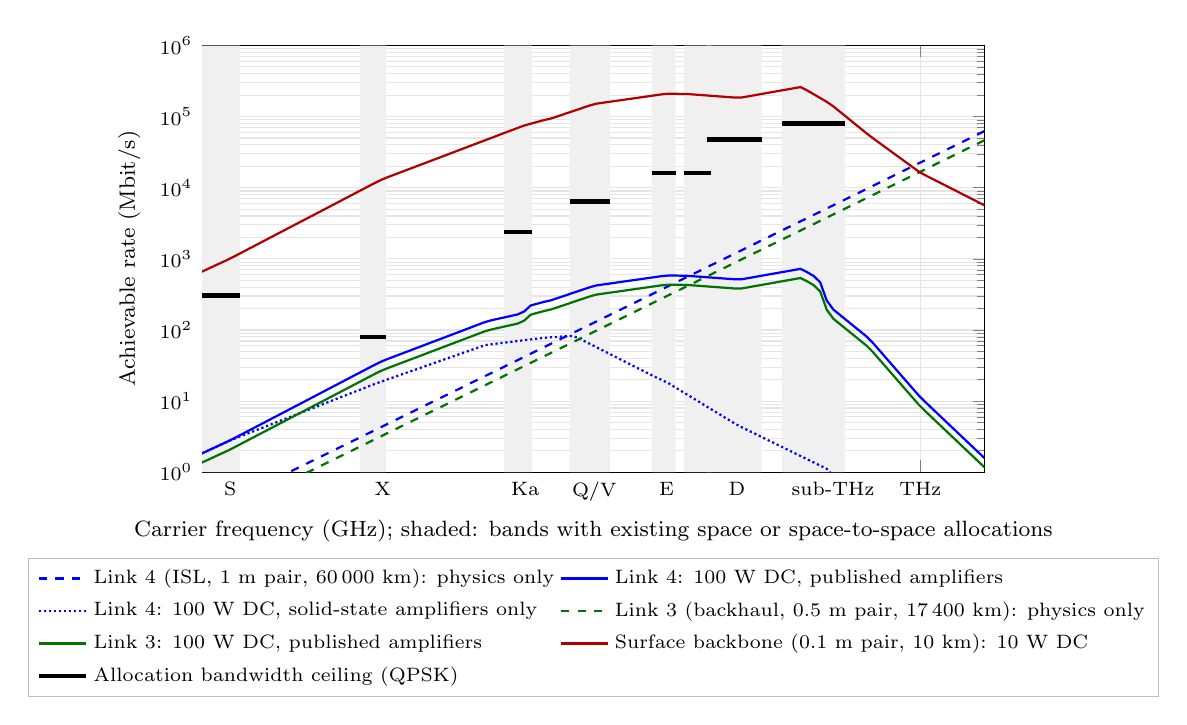
\begin{tikzpicture}
\begin{axis}[
  width=0.95\textwidth, height=7.0cm,
  xmode=log, ymode=log,
  xmin=2, xmax=1000, ymin=1, ymax=1e6,
  xlabel={Carrier frequency (GHz); shaded: bands with existing space or space-to-space allocations}, ylabel={Achievable rate (Mbit/s)},
  grid=both, grid style={gray!20},
  tick label style={font=\scriptsize}, label style={font=\footnotesize},
  legend style={font=\scriptsize, at={(0.5,-0.2)}, anchor=north, draw=gray!50, fill=white, row sep=1pt, cells={anchor=west}}, legend columns=2,
  xtick={2.5,8.4,26,45,80,140,300,600}, xticklabels={S,X,Ka,Q/V,E,D,sub-THz,THz},
]
\addplot[draw=none, fill=gray!12, forget plot] coordinates {(2,1) (2.7,1) (2.7,1e6) (2,1e6)} \closedcycle;
\addplot[draw=none, fill=gray!12, forget plot] coordinates {(7,1) (8.6,1) (8.6,1e6) (7,1e6)} \closedcycle;
\addplot[draw=none, fill=gray!12, forget plot] coordinates {(22,1) (27.5,1) (27.5,1e6) (22,1e6)} \closedcycle;
\addplot[draw=none, fill=gray!12, forget plot] coordinates {(37,1) (51,1) (51,1e6) (37,1e6)} \closedcycle;
\addplot[draw=none, fill=gray!12, forget plot] coordinates {(71,1) (86,1) (86,1e6) (71,1e6)} \closedcycle;
\addplot[draw=none, fill=gray!12, forget plot] coordinates {(92,1) (114,1) (114,1e6) (92,1e6)} \closedcycle;
\addplot[draw=none, fill=gray!12, forget plot] coordinates {(110,1) (170,1) (170,1e6) (110,1e6)} \closedcycle;
\addplot[draw=none, fill=gray!12, forget plot] coordinates {(200,1) (330,1) (330,1e6) (200,1e6)} \closedcycle;
\addplot[blue, thick, dashed] coordinates {\LFphys};
\addlegendentry{Link 4 (ISL, 1 m pair, 60\,000 km): physics only}
\addplot[blue, thick] coordinates {\LFhw};
\addlegendentry{Link 4: 100 W DC, published amplifiers}
\addplot[blue, thick, densely dotted] coordinates {\LFsspa};
\addlegendentry{Link 4: 100 W DC, solid-state amplifiers only}
\addplot[green!45!black, thick, dashed] coordinates {\LTphys};
\addlegendentry{Link 3 (backhaul, 0.5 m pair, 17\,400 km): physics only}
\addplot[green!45!black, thick] coordinates {\LThw};
\addlegendentry{Link 3: 100 W DC, published amplifiers}
\addplot[red!70!black, thick] coordinates {\BBhw};
\addlegendentry{Surface backbone (0.1 m pair, 10 km): 10 W DC}
\addplot[black, line width=1.6pt] coordinates {(2,304) (2.7,304)};
\addlegendentry{Allocation bandwidth ceiling (QPSK)}
\addplot[black, line width=1.6pt, forget plot] coordinates {(2,304) (2.7,304)};
\addplot[black, line width=1.6pt, forget plot] coordinates {(7,80) (8.6,80)};
\addplot[black, line width=1.6pt, forget plot] coordinates {(22,2400) (27.5,2400)};
\addplot[black, line width=1.6pt, forget plot] coordinates {(37,6400) (51,6400)};
\addplot[black, line width=1.6pt, forget plot] coordinates {(71,16000) (86,16000)};
\addplot[black, line width=1.6pt, forget plot] coordinates {(92,16000) (114,16000)};
\addplot[black, line width=1.6pt, forget plot] coordinates {(110,48000) (170,48000)};
\addplot[black, line width=1.6pt, forget plot] coordinates {(200,80000) (330,80000)};
\end{axis}
\end{tikzpicture}
